% ============================================================================
%  RELATÓRIO DE IMERSÃO — GRUPO 13 · ÉPSILON
%  ODS 12: Consumo e Produção Responsáveis
%  Projeto Integrador I / Design Thinking — Módulo 1
%  ETE Cícero Dias
%
%  Compilação: pdflatex (2x) — compatível com Overleaf e Google Colab.
%  Estrutura no padrão de template da disciplina (capa, folha de rosto,
%  aberturas de seção numeradas, gráficos vetoriais e referências).
% ============================================================================

\documentclass[12pt, a4paper]{article}

% ---------- Codificação e idioma ----------
\usepackage[utf8]{inputenc}
\usepackage[T1]{fontenc}
\usepackage[portuguese]{babel}
\usepackage[margin=2.5cm]{geometry}
\setlength{\headheight}{15pt}

% ---------- Tipografia ----------
% \usepackage{lmodern} % removido: nao disponivel neste ambiente
\usepackage{helvet}
\renewcommand{\familydefault}{\rmdefault}

% ---------- Recursos gráficos e tabelas ----------
\usepackage{graphicx}
\usepackage{tabularx}
\usepackage{xltabular}
\usepackage{booktabs}
\usepackage{array}
\usepackage{enumitem}
\usepackage{float}
\usepackage{caption}
\usepackage{framed}
\usepackage{lettrine}
\usepackage{ragged2e}

% ---------- Cores e gráficos vetoriais ----------
\usepackage{xcolor}
\usepackage{colortbl}
\usepackage{pgfplots}
\usepackage{pgf-pie}
\pgfplotsset{compat=1.18}

% ---------- Layout de página, capa e títulos ----------
\usepackage{tikz}
\usetikzlibrary{shadows}
\usepackage{eso-pic}
\usepackage{titlesec}
\usepackage{fancyhdr}
\usepackage{xurl}
\usepackage{hyperref}

% ============================================================================
%  PALETA DO PROJETO — Vinho/Bordô · identidade visual Grupo 13 · ÉPSILON
%  >>> Para trocar a identidade visual, ajuste APENAS as 8 cores abaixo. <<<
% ============================================================================
\definecolor{wineDeep}{HTML}{5C1A2A}    % vinho escuro — títulos e contraste
\definecolor{wine}{HTML}{7D2535}        % vinho principal — capa e cabeçalhos
\definecolor{wineSoft}{HTML}{A84B5C}    % vinho claro — números e detalhes
\definecolor{accentGold}{HTML}{C9943A}  % dourado — destaques e acentos
\definecolor{cream}{HTML}{F5F2EE}       % creme — fundos de bloco
\definecolor{creamMid}{HTML}{E8E2DC}    % creme médio — linhas de tabela
\definecolor{ink}{HTML}{1A1A1A}         % quase-preto — texto
\definecolor{slate}{HTML}{5A5A5A}       % cinza — rótulos e dados
\definecolor{corCorrecao}{HTML}{B02A26}
\definecolor{corCorrecaoBg}{HTML}{FAEDEC}

% ---------- Hyperlinks ----------
\hypersetup{
    colorlinks=true,
    linkcolor=wineDeep,
    filecolor=wineDeep,
    urlcolor=wine,
    citecolor=wine,
    breaklinks=true
}

% ============================================================================
%  DADOS DO TRABALHO
% ============================================================================
\newcommand{\projTitulo}{ÉPSILON}
\newcommand{\projSubtitulo}{Plataforma para consumo consciente e transparência de preços}
\newcommand{\projODS}{ODS 12 \textemdash{} Consumo e Produção Responsáveis}
\newcommand{\projGrupo}{Grupo 13}
\newcommand{\projCurso}{Técnico em Desenvolvimento de Sistemas}
\newcommand{\projModulo}{Módulo 1}
\newcommand{\projDisciplina}{Design Thinking \textbullet\ Projeto Integrador I}
\newcommand{\projProfessora}{Profa. Samara Silvia Sabino}
\newcommand{\projInstituicao}{ETE Cícero Dias}
\newcommand{\projEtapa}{Memorial de Projeto}
\newcommand{\projData}{Recife, Junho de 2026}

% ---------- Logos ----------
\newcommand{\logoETE}{
\includegraphics[height=1.5cm]{imgs/logoETE.png}}
\newcommand{\logoNAVE}{
\includegraphics[height=1.5cm]{imgs/logoNAVE.png}}

% ============================================================================
%  ESTILO DAS ABERTURAS DE SEÇÃO
% ============================================================================
\titleformat{\section}[display]
  {\normalfont\sffamily}
  {\flushright\fontsize{84}{84}\selectfont\bfseries\color{wineSoft}\thesection}
  {6pt}
  {\Huge\bfseries\color{wineDeep}\filright}
\titlespacing*{\section}{0pt}{0pt}{30pt}

\titleformat{\subsection}
  {\normalfont\sffamily\large\bfseries\color{wineDeep}}
  {\thesubsection}{0.6em}{}
\titlespacing*{\subsection}{0pt}{16pt}{6pt}

\newcommand{\novaSecao}[1]{\clearpage\vspace*{2.2cm}\section{#1}}

% ---------- Cabeçalho e rodapé ----------
\fancypagestyle{corpo}{%
  \fancyhf{}
  \renewcommand{\headrulewidth}{0.6pt}
  \renewcommand{\headrule}{\hbox to\headwidth{\color{wine}\leaders\hrule height \headrulewidth\hfill}}
  \fancyhead[L]{\footnotesize\sffamily\textcolor{wineDeep}{\textbf{ÉPSILON}}\ \textcolor{slate}{\textperiodcentered\ \projInstituicao}}
  \fancyhead[R]{\footnotesize\sffamily\textcolor{slate}{Memorial de Projeto \textperiodcentered\ Design Thinking}}
  \fancyfoot[L]{\footnotesize\sffamily\textcolor{slate}{\projODS}}
  \fancyfoot[R]{\footnotesize\sffamily\textcolor{wineDeep}{\textbf{\thepage}}}
}

% ---------- Caixa de citação ----------
\newenvironment{citacaoBox}{%
  \par\vspace{6pt}%
  \def\FrameCommand{{\color{wineSoft}\vrule width 2pt}\hspace{12pt}}%
  \MakeFramed{\advance\hsize-\width\FrameRestore}%
  \small\itshape\color{ink}%
}{%
  \par\endMakeFramed\vspace{6pt}%
}
\newcommand{\citacaoDestaque}[2]{%
  \begin{citacaoBox}#1\par\vspace{4pt}%
    {\normalfont\footnotesize\color{slate}\hfill\textsc{\textemdash{}\,#2}}%
  \end{citacaoBox}%
}

% ---------- Anotações de correção ----------
\newif\ifmostrarcorrecoes
\mostrarcorrecoestrue
\newcommand{\correcao}[1]{%
  \ifmostrarcorrecoes
    \par\vspace{6pt}\noindent
    \setlength{\fboxsep}{9pt}%
    \fcolorbox{corCorrecao}{corCorrecaoBg}{%
      \begin{minipage}{\dimexpr\linewidth-2\fboxsep-2\fboxrule\relax}
        {\sffamily\bfseries\footnotesize\color{corCorrecao}\textsf{CORREÇÃO \textemdash{} PROFA. SAMARA}}\par\vspace{3pt}
        {\normalfont\small\color{corCorrecao} #1}
      \end{minipage}}%
    \par\vspace{6pt}
  \fi
}

% ---------- Legenda de gráficos ----------
\newcommand{\swatch}[1]{\raisebox{0.5pt}{\tikz{\fill[#1] (0,0) rectangle (9pt,9pt);}}}
\newcommand{\legendaItem}[2]{%
  \noindent\swatch{#1}\hspace{6pt}\begin{minipage}[t]{\dimexpr\linewidth-18pt\relax}#2\end{minipage}\par\vspace{3pt}%
}

% ---------- Banner de imagem ----------
\newcommand{\bannerImg}[2][5.6cm]{%
  \noindent\begin{tikzpicture}
    \clip (0,0) rectangle (\linewidth,#1);
    \node[anchor=center, inner sep=0] at (0.5\linewidth, 0.5*#1) {\includegraphics[width=\linewidth]{#2}};
    \draw[cream, line width=0.8pt] (0,0) rectangle (\linewidth,#1);
  \end{tikzpicture}\par
}

\setlength{\parskip}{6pt}
\setlength{\parindent}{0pt}

\begin{document}

% ============================================================================
%  CAPA
% ============================================================================
\begin{titlepage}
\thispagestyle{empty}
\begin{tikzpicture}[remember picture, overlay]
  % --- Imagem de capa ---
  \begin{scope}
    \clip (current page.south west) rectangle (current page.north east);
    \node at (current page.center) {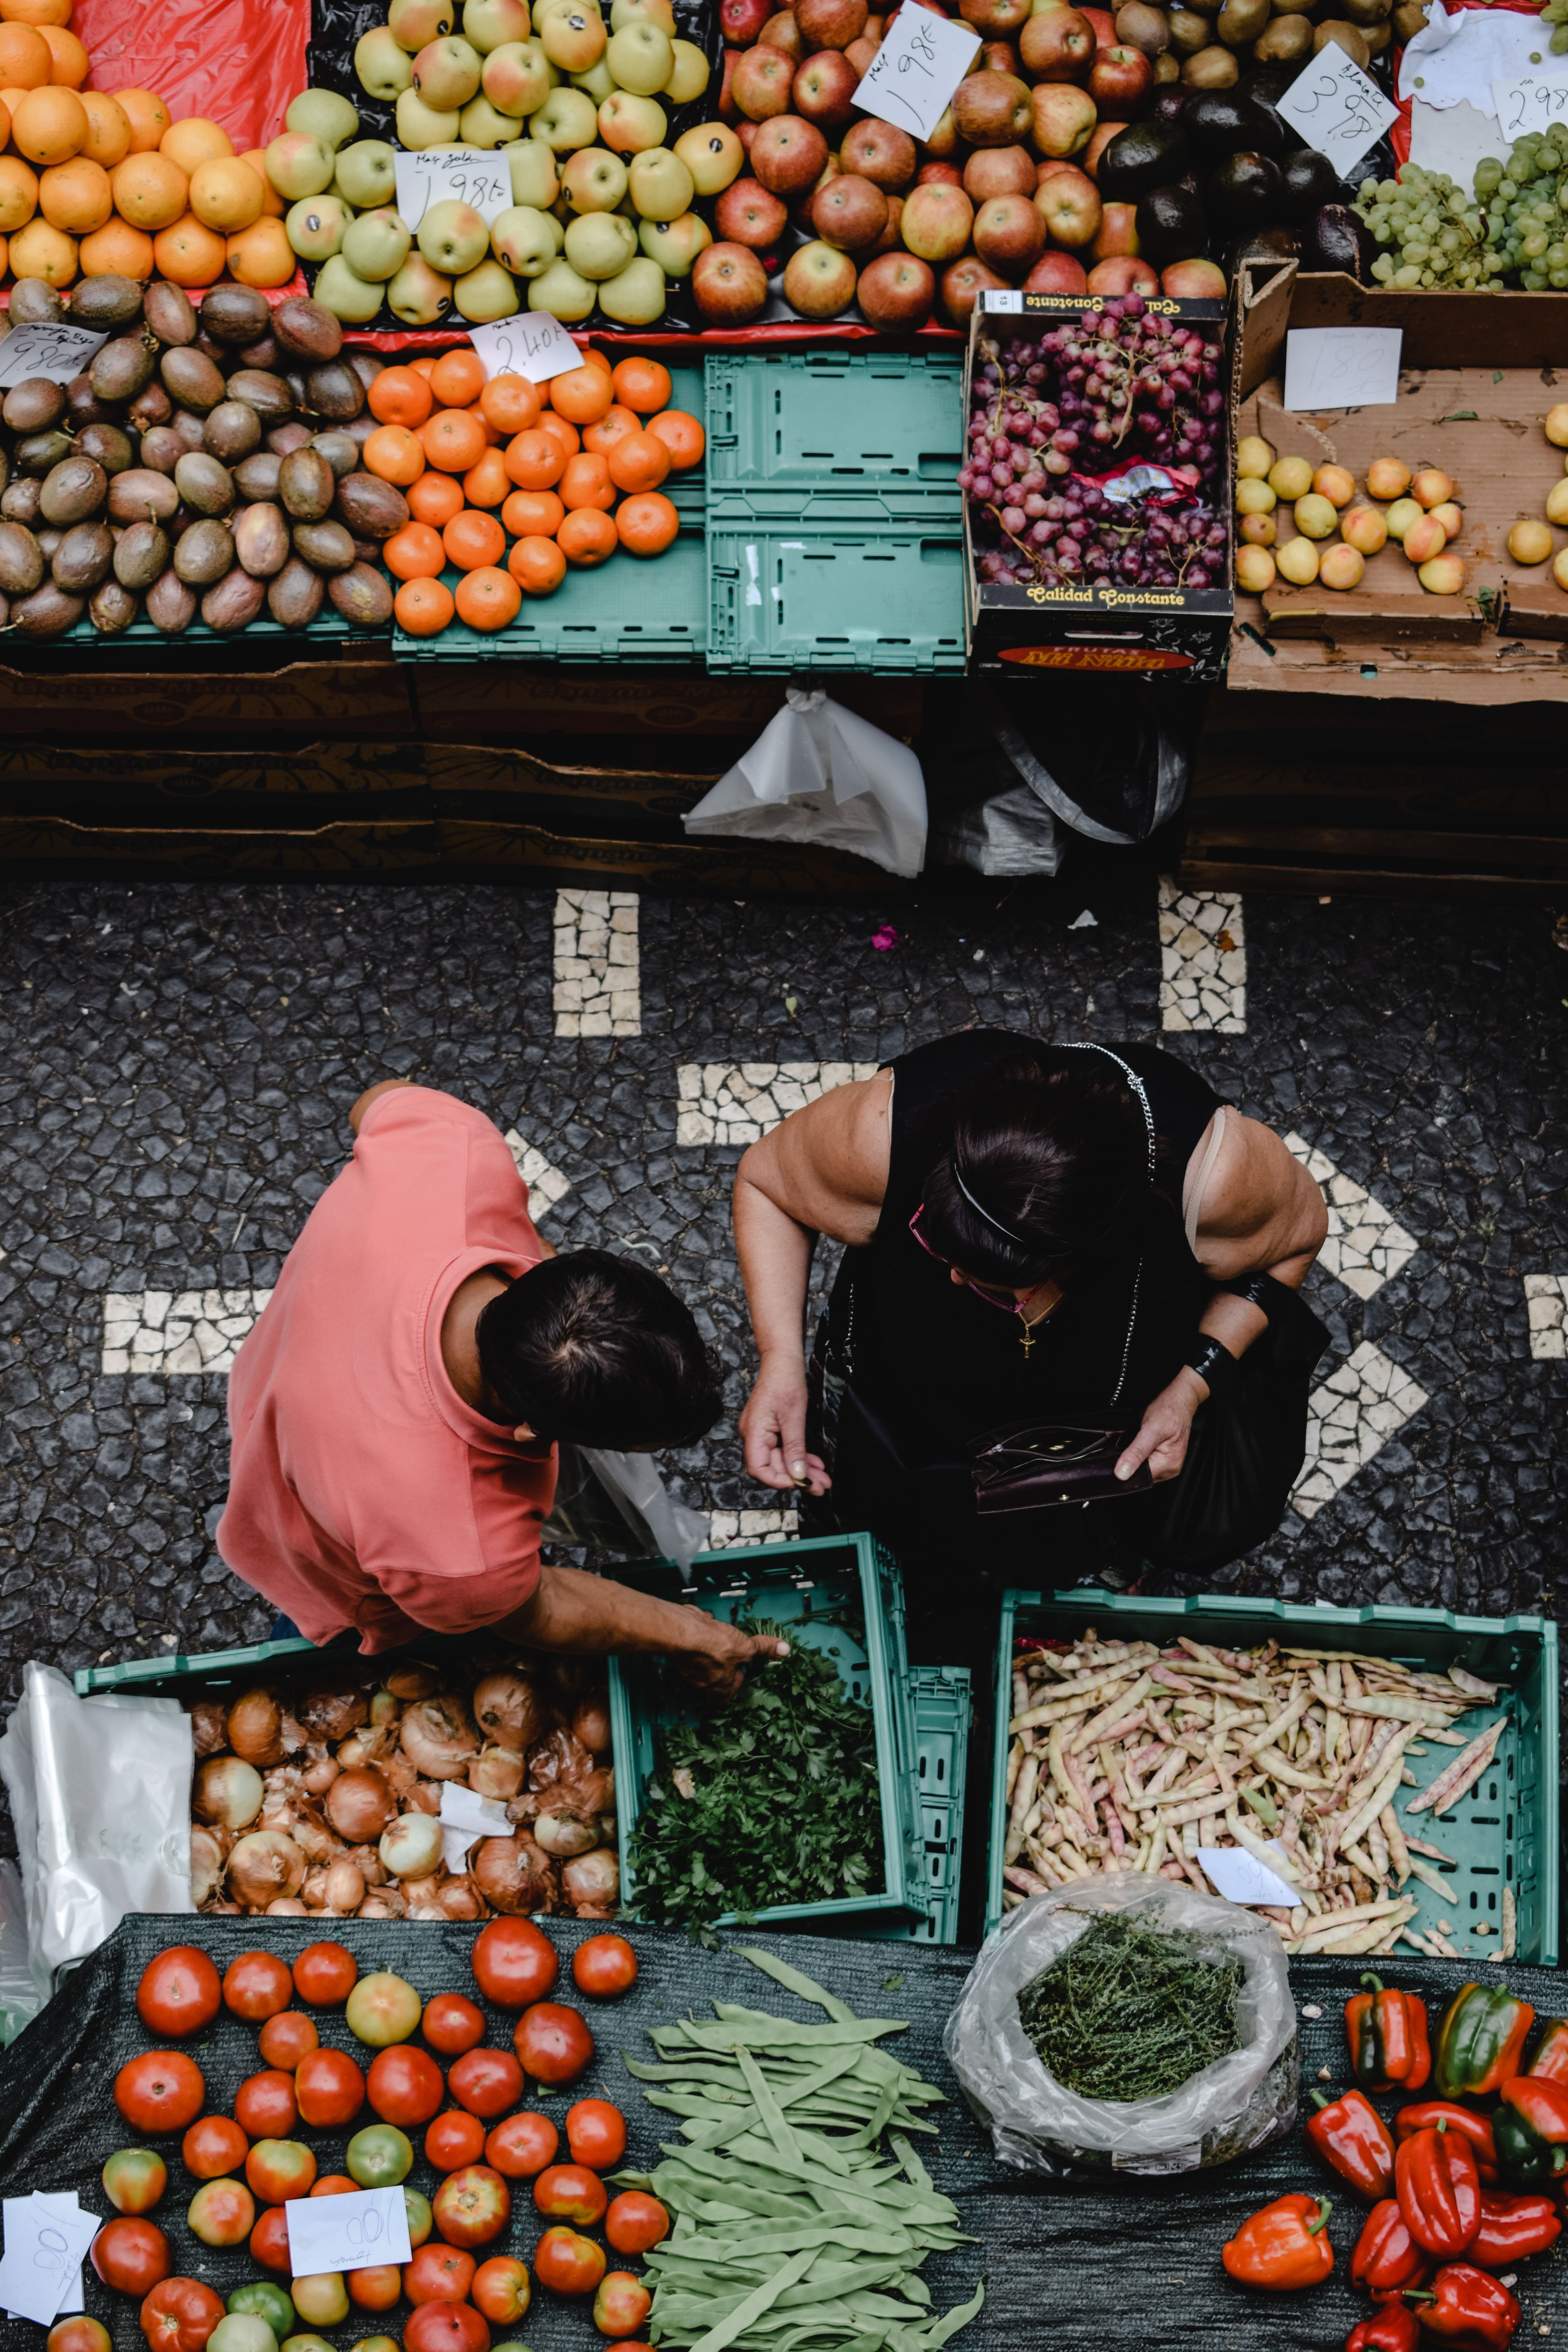
\includegraphics[width=\paperwidth]{imgs/capa.jpg}};
  \end{scope}

  % --- Escurecimento em camadas ---
  \fill[black, opacity=0.22] (current page.south west) rectangle ([yshift=9.5cm]current page.south east);
  \fill[black, opacity=0.30] (current page.south west) rectangle ([yshift=6.0cm]current page.south east);
  \fill[black, opacity=0.45] (current page.south west) rectangle ([yshift=3.2cm]current page.south east);
  \fill[black, opacity=0.26] (current page.north west) rectangle ([yshift=-2.7cm]current page.north east);

  % --- Faixa de cor vinho no topo ---
  \fill[wine, opacity=0.82]
    (current page.north west) rectangle ([yshift=-2.1cm]current page.north east);

  % --- Moldura fina ---
  \draw[cream, line width=0.6pt]
    ([shift={(0.9cm,0.9cm)}]current page.south west)
    rectangle ([shift={(-0.9cm,-0.9cm)}]current page.north east);

  % --- Topo: instituição (sobre a faixa vinho) ---
  \node[anchor=north, text=cream, font=\sffamily] at ([yshift=-1.7cm]current page.north)
    {\small ETE CÍCERO DIAS \ \textbullet\ \ NAVE};

  % --- Bloco de título ---
  \node[anchor=south west, text=white, align=left] at ([shift={(1.7cm,4.0cm)}]current page.south west)
    {\sffamily\bfseries\fontsize{82}{82}\selectfont ÉPSILON};
  \node[anchor=north west, text=cream, align=left, text width=15.5cm] at ([shift={(1.8cm,3.6cm)}]current page.south west)
    {\sffamily\large \projSubtitulo};

  % --- Linha + metadados ---
  \draw[accentGold, line width=0.7pt]
    ([shift={(1.8cm,2.75cm)}]current page.south west) -- ([shift={(9.5cm,2.75cm)}]current page.south west);
  \node[anchor=north west, text=cream, align=left] at ([shift={(1.8cm,2.55cm)}]current page.south west)
    {\sffamily\footnotesize MEMORIAL DE PROJETO \ \textbullet\ \ ODS 12 \ \textbullet\ \ GRUPO 13};
\end{tikzpicture}
\end{titlepage}

% ============================================================================
%  FOLHA DE ROSTO
% ============================================================================
\thispagestyle{empty}
\vspace*{2.2cm}
\begin{center}
  {\logoETE\hspace{1.4cm}\logoNAVE}\\[2.4cm]

  {\sffamily\footnotesize\color{slate} \MakeUppercase{\projODS}}\\[0.45cm]
  {\color{wineSoft}\rule{2.4cm}{1.2pt}}\\[1.0cm]

  {\sffamily\bfseries\color{ink}\fontsize{56}{56}\selectfont \projTitulo}\\[0.55cm]
  {\itshape\large\color{wineDeep} \projSubtitulo}\\[2.6cm]

  {\sffamily\color{slate}\large \projGrupo \quad\textperiodcentered\quad \projModulo}\\[0.55cm]
  {\color{ink} Equipe ÉPSILON}
\end{center}

\vfill

\begin{center}
  {\color{wineSoft}\rule{0.42\textwidth}{0.5pt}}\\[0.7cm]
  {\sffamily\footnotesize\color{slate}
    \projInstituicao \ \textbullet\ \ \projCurso\\[3pt]
    \projDisciplina\\[3pt]
    \projProfessora \quad\textperiodcentered\quad \projEtapa\\[3pt]
    \projData}
\end{center}
\vspace{1.2cm}
\clearpage

% ============================================================================
%  PÁGINA DA EQUIPE
% ============================================================================
\thispagestyle{empty}
\vspace*{1.5cm}
\begin{center}
  {\logoETE\hspace{1.4cm}\logoNAVE}\\[1.2cm]
  {\sffamily\bfseries\color{wineDeep}\fontsize{34}{34}\selectfont \projTitulo}\\[0.25cm]
  {\sffamily\color{slate}\large Equipe \textbullet\ \projGrupo\ \textbullet\ \projModulo}\\[1.5cm]

  \newcommand{\membro}[1]{%
    \begin{minipage}[t]{3.7cm}\centering
      \setlength{\fboxsep}{0pt}%
      \fcolorbox{wineSoft}{cream}{\parbox[c][4.7cm][c]{3.7cm}{\centering\color{slate}\scriptsize\itshape [ foto ]}}\\[6pt]
      {\sffamily\small\color{ink} #1}
    \end{minipage}}

  \membro{Nome Integrante 1}\hspace{0.55cm}%
  \membro{Nome Integrante 2}\hspace{0.55cm}%
  \membro{Nome Integrante 3}\\[0.95cm]
  \membro{Nome Integrante 4}\hspace{0.55cm}%
  \membro{Nome Integrante 5}
\end{center}
\clearpage

% ============================================================================
%  PÁGINA DA PROFESSORA
% ============================================================================
\thispagestyle{empty}
\newcommand{\duracaoProjeto}{1º de abril a 1º de junho de 2026}
\vspace*{1.0cm}

{\centering\sffamily\footnotesize\color{wine} NOTA DA PROFESSORA\par}
\vspace{0.28cm}
{\centering\sffamily\bfseries\fontsize{36}{36}\selectfont\color{ink} O Desafio\par}
\vspace{0.28cm}
{\centering{\color{wineSoft}\rule{2.6cm}{1.2pt}}\par}
\vspace{0.7cm}

\begin{center}
\begin{minipage}{0.82\textwidth}
{\centering\itshape\large\color{wineDeep} Aprender resolvendo problemas reais: por que um desafio como este vale mais do que uma prova.\par}
\vspace{0.55cm}

\setlength{\parskip}{6pt}
\color{ink}
Este memorial documenta um \textbf{projeto integrador} conduzido pelo método do \textbf{Design Thinking}. Partindo de um dos Objetivos de Desenvolvimento Sustentável (ODS) da ONU, cada grupo identifica um problema real, investiga-o a fundo nas etapas de Imersão e Definição e chega à proposta de um protótipo. Não é um exercício teórico: é a vivência completa de como uma ideia se transforma em solução, conduzida ao longo de cerca de dois meses (\duracaoProjeto).

Do ponto de vista \textbf{pedagógico}, o desafio coloca o estudante no centro da própria aprendizagem. Em vez de receber respostas prontas, ele formula perguntas, coleta dados, erra, refaz e defende suas escolhas. Essa aprendizagem ativa desenvolve pensamento crítico, empatia com o usuário, trabalho em equipe e autonomia \textemdash{} competências que nenhuma prova tradicional consegue medir.

Do ponto de vista \textbf{mercadológico}, é exatamente assim que se trabalha no mundo real. Pesquisa de usuário, definição de problema, prototipação e validação são as etapas de qualquer time de produto, design ou tecnologia. Ao terminar, o estudante não leva apenas uma nota: leva um caso documentado, material de portfólio e a experiência concreta que o mercado procura.
\end{minipage}
\end{center}

\vspace{1.2cm}
\begin{center}
  {\color{creamMid}\rule{0.35\textwidth}{0.6pt}}\\[0.5cm]
  \begin{tikzpicture}
    \node[circle, draw=wineSoft, line width=1.5pt, minimum size=3.0cm, inner sep=0,
          path picture={\node at (path picture bounding box.center)
            {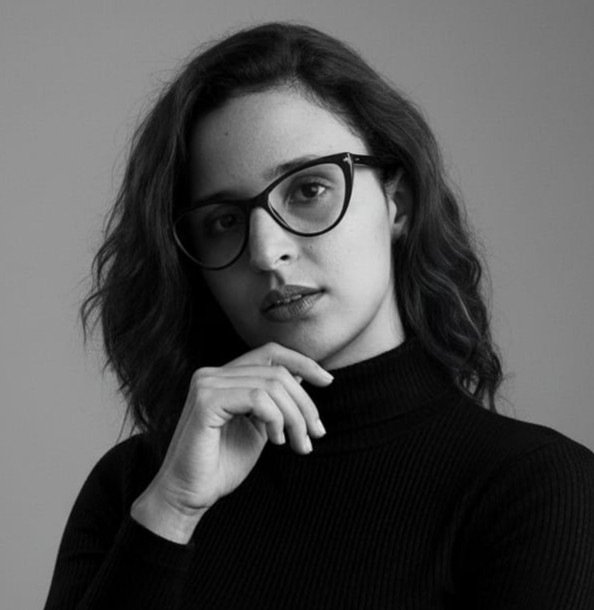
\includegraphics[width=3.3cm]{imgs/avatar-samara.jpg}};}] {};
  \end{tikzpicture}\\[0.4cm]
  {\sffamily\bfseries\color{wineDeep} Profa. Samara Silvia Sabino}\\[3pt]
  {\sffamily\footnotesize\color{slate} Design Thinking \textperiodcentered\ Projeto Integrador \textperiodcentered\ ETE Cícero Dias}\\[2pt]
  {\sffamily\footnotesize\color{slate} \duracaoProjeto}
\end{center}
\vspace{0.9cm}
\clearpage

% ============================================================================
%  RESUMO · PALAVRAS-CHAVE · DESTAQUES
% ============================================================================
\pagestyle{corpo}

\begin{center}
  {\sffamily\large\color{wineDeep} \MakeUppercase{Resumo}}\\[3pt]
  {\color{wineSoft}\rule{1.8cm}{1pt}}
\end{center}
\vspace{0.5cm}

{\color{ink}
\lettrine[lines=3, lhang=0.08, findent=3pt, nindent=8pt]{\color{wineDeep}\sffamily O}{} projeto ÉPSILON investiga como consumidores da Região Metropolitana do Recife enfrentam dificuldades para realizar compras mais conscientes e economicamente vantajosas. A ausência de ferramentas simples para acompanhar a evolução de preços, identificar promoções reais e planejar compras de forma sustentável contribui para decisões impulsivas, desperdício de recursos financeiros e práticas de consumo pouco alinhadas aos princípios da ODS 12. Por meio de Pesquisa Desk, formulário online aplicado a 25 participantes e entrevistas semiestruturadas, o grupo mapeou as principais dores, comportamentos e expectativas dos consumidores. Os resultados revelaram que o alto preço de produtos sustentáveis, a falta de transparência nas informações e a dificuldade de comparar preços são os maiores obstáculos para um consumo responsável. A proposta do grupo é uma plataforma digital capaz de acompanhar a variação de preços ao longo do tempo, apoiar o planejamento financeiro e incentivar decisões de compra mais conscientes.
\par}

\vspace{6pt}
\noindent\textbf{Palavras-chave:} Consumo consciente; Transparência de preços; ODS 12; Design Thinking; Plataforma digital; Planejamento financeiro; Sustentabilidade.

\vspace{10pt}
\noindent{\sffamily\bfseries\color{wineDeep} Destaques}
\vspace{2pt}

\begin{itemize}[leftmargin=1.2em, itemsep=4pt, label=\textcolor{wineSoft}{\textbf{\textbullet}}]
  \item 64\% dos entrevistados apontam o alto preço dos produtos sustentáveis como principal barreira ao consumo responsável.
  \item 44\% dos participantes realizam compras por impulso, especialmente quando encontram promoções.
  \item A ausência de histórico de preços dificulta a identificação de ofertas realmente vantajosas.
  \item 68\% dos respondentes já reutilizam embalagens, demonstrando predisposição a hábitos mais sustentáveis.
  \item Acesso à informação clara e confiável é o principal fator para decisões de compra mais conscientes.
\end{itemize}

% ============================================================================
%  SUMÁRIO
% ============================================================================
\clearpage
\vspace*{0.4cm}
{\sffamily\bfseries\fontsize{34}{34}\selectfont\color{wineDeep} Sumário}\par
\vspace{4pt}{\color{wine}\rule{\linewidth}{1.5pt}}\par
\vspace{0.8cm}
\setcounter{tocdepth}{2}
\makeatletter
\@starttoc{toc}
\makeatother

% ============================================================================
%  1. INTRODUÇÃO
% ============================================================================
\clearpage
\bannerImg{imgs/intro.jpg}
\vspace{0.5cm}
\section{Introdução}

Os Objetivos de Desenvolvimento Sustentável (ODS), estabelecidos pela Organização das Nações Unidas (ONU), representam um conjunto de metas globais voltadas para a promoção do desenvolvimento econômico, social e ambiental de forma equilibrada. Entre esses objetivos, destaca-se a \textbf{ODS 12 \textemdash{} Consumo e Produção Responsáveis}, que busca incentivar padrões sustentáveis de consumo, reduzir desperdícios e promover o uso eficiente dos recursos naturais.

No contexto atual, consumidores enfrentam desafios relacionados à transparência das informações de mercado, especialmente no acompanhamento da variação de preços de produtos e serviços. A dificuldade de identificar promoções reais, comparar valores entre estabelecimentos e planejar compras de maneira eficiente pode contribuir para decisões impulsivas, desperdício de recursos financeiros e práticas de consumo pouco sustentáveis.

Diante desse cenário, a Equipe ÉPSILON desenvolveu um processo de imersão utilizando os princípios do \textbf{Design Thinking} com o objetivo de compreender o comportamento dos consumidores, identificar suas principais dores e investigar oportunidades de melhoria relacionadas ao consumo consciente. A pesquisa concentrou-se na análise da relação entre informação, preço e tomada de decisão durante o processo de compra.

Para a obtenção dos dados, foram empregadas diferentes técnicas de investigação, incluindo Pesquisa Desk, aplicação de questionário online por meio do Google Forms e entrevistas semiestruturadas gravadas. Essas abordagens permitiram coletar informações quantitativas e qualitativas sobre hábitos de consumo, dificuldades enfrentadas pelos usuários e percepções relacionadas ao consumo sustentável.

Os resultados obtidos evidenciaram que fatores como a falta de informação, a dificuldade de acompanhar a evolução dos preços e o alto custo de produtos considerados sustentáveis influenciam diretamente as decisões dos consumidores. Com base nesses achados, o projeto propõe o desenvolvimento de uma solução tecnológica capaz de acompanhar a variação dos preços ao longo do tempo, fornecer informações confiáveis aos consumidores e apoiar decisões de compra mais conscientes.

% ============================================================================
%  2. METODOLOGIA
% ============================================================================
\novaSecao{Metodologia}

\subsection{Matriz de Alinhamento}

Para garantir que o projeto estivesse focado no escopo e no desafio corretos, os parâmetros de alinhamento foram definidos da seguinte forma:

\renewcommand{\arraystretch}{1.45}
\begingroup
\small
\begin{xltabular}{\textwidth}{!{\color{wineSoft}\vrule}>{\bfseries\color{wineDeep}\raggedright\arraybackslash}p{4.1cm}!{\color{wineSoft}\vrule}X!{\color{wineSoft}\vrule}}
\arrayrulecolor{wineSoft}\hline
\rowcolor{wine}\multicolumn{2}{!{\color{wineSoft}\vrule}c!{\color{wineSoft}\vrule}}{\textcolor{white}{\sffamily\bfseries IDENTIFICAÇÃO}}\\ \hline
Nome / Número do Grupo & ÉPSILON / Grupo 13 \\ \hline
Integrantes & Nome Integrante 1, Nome Integrante 2, Nome Integrante 3, Nome Integrante 4, Nome Integrante 5. \\ \hline
ODS Escolhida & ODS 12 \textemdash{} Consumo e Produção Responsáveis \\ \hline
\rowcolor{wine}\multicolumn{2}{!{\color{wineSoft}\vrule}c!{\color{wineSoft}\vrule}}{\textcolor{white}{\sffamily\bfseries IMERSÃO}}\\ \hline
Quem pode estar sendo afetado? & Consumidores da Região Metropolitana do Recife que realizam compras em estabelecimentos varejistas e atacadistas, além de pequenos comerciantes e distribuidores envolvidos na cadeia de consumo. \\ \hline
O que o grupo quer descobrir? & Como os consumidores acompanham preços, identificam promoções, tomam decisões de compra e quais dificuldades enfrentam para adotar práticas de consumo mais conscientes e sustentáveis. \\ \hline
Quais técnicas de imersão planejam usar? & Pesquisa Desk (pesquisa documental), Questionário Online (Google Forms) e Entrevista Semiestruturada gravada. \\ \hline
\rowcolor{wine}\multicolumn{2}{!{\color{wineSoft}\vrule}c!{\color{wineSoft}\vrule}}{\textcolor{white}{\sffamily\bfseries ESCOPO}}\\ \hline
O que está DENTRO do escopo? & Hábitos de consumo, comportamento do consumidor, transparência de preços, consumo consciente, desperdício de recursos, práticas sustentáveis e acompanhamento da variação de preços de produtos. \\ \hline
O que está FORA do escopo? & Produção industrial em larga escala, gestão interna de fabricantes, políticas governamentais de tributação, logística internacional e problemas ambientais sem relação direta com o comportamento de consumo analisado. \\ \hline
Hipótese de solução (ideia inicial) & Uma plataforma digital capaz de acompanhar a evolução dos preços de produtos ao longo do tempo, auxiliando consumidores na identificação de promoções reais e incentivando decisões de compra mais conscientes. \\ \hline
Resultado esperado da imersão & Compreender as dores, necessidades e comportamentos dos consumidores para fundamentar a definição do problema e orientar o desenvolvimento da solução tecnológica. \\ \hline
\end{xltabular}
\endgroup

\subsection{Matriz CSD}

Este quadro ajuda a visualizar o que o grupo já domina e tem certeza de como fazer, as suposições sobre tudo que engloba o projeto e as dúvidas que ainda restam \textemdash{} sendo estas últimas o guia principal da pesquisa de campo.

\renewcommand{\arraystretch}{1.4}
\begingroup
\small
\begin{xltabular}{\textwidth}{!{\color{wineSoft}\vrule}X!{\color{wineSoft}\vrule}X!{\color{wineSoft}\vrule}X!{\color{wineSoft}\vrule}}
\arrayrulecolor{wineSoft}\hline
\rowcolor{wine}\multicolumn{3}{!{\color{wineSoft}\vrule}c!{\color{wineSoft}\vrule}}{\textcolor{white}{\sffamily\bfseries MATRIZ CSD \textemdash{} ÉPSILON}}\\ \hline
\rowcolor{creamMid}
\centering\textbf{CERTEZAS} & \centering\textbf{SUPOSIÇÕES} & \centering\arraybackslash\textbf{DÚVIDAS} \\
\rowcolor{cream}
\centering\footnotesize\textit{O que é fato ou base do projeto} & \centering\footnotesize\textit{O que achamos que é verdade, mas precisamos validar} & \centering\arraybackslash\footnotesize\textit{Perguntas que a Pesquisa Desk deve responder} \\ \hline
\endhead
O acesso à informação é fundamental para decisões de consumo mais conscientes.
& Consumidores estariam dispostos a usar uma plataforma de monitoramento de preços no dia a dia.
& Existem ferramentas gratuitas e acessíveis de acompanhamento de preços disponíveis no Brasil? \\ \hline
O preço elevado de produtos sustentáveis é uma barreira real para grande parte dos consumidores.
& A gamificação (pontuação por boas escolhas de consumo) poderia engajar usuários na plataforma.
& Qual seria o modelo de negócio viável para manter a plataforma sem comprometer a neutralidade das informações? \\ \hline
Compras impulsivas são favorecidas pela ausência de histórico e comparação de preços.
& Consumidores confiariam mais em uma plataforma colaborativa do que em dados fornecidos pelas próprias marcas.
& Como garantir a atualização constante e a confiabilidade dos dados de preço coletados? \\ \hline
A maioria dos consumidores já adota alguma prática de redução de desperdício (lista de compras, reaproveitamento).
& Integrar alertas de preço via WhatsApp ou notificação aumentaria a retenção de usuários.
& Quais são as regulamentações brasileiras sobre divulgação de preços no varejo? \\ \hline
\end{xltabular}
\endgroup

\subsection{Técnicas de Imersão e Justificativa}

A etapa de imersão utilizou três técnicas complementares de pesquisa: Pesquisa Desk, Questionário Online e Entrevista Semiestruturada. A combinação dessas abordagens permitiu coletar dados quantitativos e qualitativos, proporcionando uma visão mais abrangente do problema investigado.

A \textbf{Pesquisa Desk} foi utilizada para levantar informações em artigos científicos, relatórios institucionais e publicações relacionadas à ODS 12, ao consumo consciente e ao comportamento do consumidor, fornecendo embasamento teórico para a investigação.

O \textbf{Questionário Online} (Google Forms) foi escolhido por permitir ampla distribuição e fácil acesso, possibilitando coletar informações de forma rápida e anônima sobre hábitos de consumo, percepção sobre sustentabilidade e critérios de decisão de compra.

A \textbf{Entrevista Semiestruturada Gravada} aprofundou aspectos não capturáveis por perguntas fechadas, explorando experiências pessoais e dificuldades reais em situações de consumo, contribuindo para a construção das personas e mapas de empatia.

% ============================================================================
%  3. PESQUISA DESK
% ============================================================================
\novaSecao{Pesquisa Desk}

A Pesquisa Desk constituiu a primeira etapa da imersão e teve como objetivo reunir informações secundárias relevantes para compreender o cenário do consumo consciente, da produção responsável e da relação entre consumidores, fornecedores e mercado varejista. O levantamento bibliográfico contemplou artigos científicos, relatórios institucionais e publicações acadêmicas relacionados à ODS 12, abrangendo principalmente estudos publicados entre 2020 e 2026.

Os resultados evidenciaram que o acesso à informação exerce papel fundamental na promoção do consumo responsável. Diversos estudos apontam que consumidores tendem a tomar decisões mais conscientes quando possuem acesso facilitado a informações sobre preços, origem dos produtos, impactos ambientais e alternativas de consumo sustentável.

Outro aspecto recorrente identificado na literatura refere-se à influência do fator econômico sobre o comportamento do consumidor. Embora exista crescente interesse por produtos sustentáveis, o preço continua sendo uma das principais barreiras para sua adoção em larga escala \textemdash{} constatação que se confirmou nos dados da pesquisa de campo.

\subsection{Principais Insights da Pesquisa Desk}

\begin{itemize}[leftmargin=1.4em, itemsep=8pt, label=\textcolor{wineSoft}{\textbf{\textbullet}}]
  \item \textbf{Informação como ferramenta de consumo consciente:} consumidores tomam decisões mais responsáveis quando possuem acesso a informações claras e confiáveis sobre produtos e preços.
  \item \textbf{Preço como principal barreira:} o custo elevado de produtos sustentáveis ainda representa um dos maiores obstáculos para a adoção de práticas de consumo responsável.
  \item \textbf{Importância da transparência:} a divulgação clara de preços e características dos produtos favorece a tomada de decisão consciente.
  \item \textbf{Tecnologia como facilitadora:} plataformas digitais podem auxiliar consumidores no monitoramento de preços, planejamento financeiro e redução de desperdícios.
  \item \textbf{ODS 12 como referência estratégica:} iniciativas voltadas para consumo e produção responsáveis contribuem para o desenvolvimento sustentável e para a conscientização da população.
\end{itemize}

% ============================================================================
%  4. PESQUISA PRIMÁRIA
% ============================================================================
\novaSecao{Pesquisa Primária}

\subsection{Entrevista Semiestruturada}

A entrevista semiestruturada gravada foi aplicada para aprofundar aspectos que não poderiam ser completamente compreendidos por meio de perguntas objetivas. A técnica permitiu explorar experiências pessoais, percepções e dificuldades enfrentadas pelos participantes em situações reais de consumo, contribuindo diretamente para a construção das personas e mapas de empatia apresentados na etapa de Definição.

\subsection{Formulário}

O formulário online permaneceu disponível por aproximadamente 10 dias, alcançando uma amostra válida de 25 consumidores residentes na Região Metropolitana do Recife. O objetivo foi compreender hábitos de consumo, percepções sobre sustentabilidade, dificuldades para adoção de práticas conscientes e fatores que influenciam a tomada de decisão nas compras.

% ---------- GRÁFICO: Gênero ----------
\begin{figure}[H]
\centering
\caption{Distribuição dos participantes por gênero. \\ \small Amostra: 25 pessoas que responderam via internet}\label{fig:genero}
\vspace{4pt}
\begin{tikzpicture}
\pie[radius=2, color={wine, wineSoft}, text=,
     every only number node/.style={text=white, font=\footnotesize\bfseries}]{52, 48}
\end{tikzpicture}
\vspace{8pt}

\begin{minipage}{0.92\textwidth}\footnotesize
\legendaItem{wine}{\textbf{52\%} \textemdash{} Feminino}
\legendaItem{wineSoft}{\textbf{48\%} \textemdash{} Masculino}
\end{minipage}
\end{figure}

% ---------- GRÁFICO: Principais dificuldades ----------
\begin{figure}[H]
\centering
\caption{Principais dificuldades para um consumo sustentável. \\ \small Amostra: 25 pessoas que responderam via internet}\label{fig:dificuldades}
\vspace{4pt}
\begin{tikzpicture}
\pie[radius=2, color={wine, wineSoft, accentGold, slate}, text=,
     every only number node/.style={text=white, font=\footnotesize\bfseries}]{64, 40, 28, 8}
\end{tikzpicture}
\vspace{8pt}

\begin{minipage}{0.92\textwidth}\footnotesize
\legendaItem{wine}{\textbf{64\%} \textemdash{} Alto preço dos produtos sustentáveis}
\legendaItem{wineSoft}{\textbf{40\%} \textemdash{} Falta de hábito}
\legendaItem{accentGold}{\textbf{28\%} \textemdash{} Falta de informação}
\legendaItem{slate}{\textbf{8\%} \textemdash{} Outros}
\end{minipage}
\end{figure}

% ---------- GRÁFICO: Compras por impulso ----------
\begin{figure}[H]
\centering
\caption{Com que frequência você realiza compras por impulso? \\ \small Amostra: 25 pessoas que responderam via internet}\label{fig:impulso}
\vspace{4pt}
\begin{tikzpicture}
\pie[radius=2, color={wine, wineSoft, accentGold, slate}, text=,
     every only number node/.style={text=white, font=\footnotesize\bfseries}]{44, 28, 16, 12}
\end{tikzpicture}
\vspace{8pt}

\begin{minipage}{0.92\textwidth}\footnotesize
\legendaItem{wine}{\textbf{44\%} \textemdash{} Às vezes, especialmente quando encontro promoções}
\legendaItem{wineSoft}{\textbf{28\%} \textemdash{} Raramente}
\legendaItem{accentGold}{\textbf{16\%} \textemdash{} Frequentemente}
\legendaItem{slate}{\textbf{12\%} \textemdash{} Nunca, compro apenas o planejado}
\end{minipage}
\end{figure}

% ---------- GRÁFICO: Reutilização ----------
\begin{figure}[H]
\centering
\caption{Você costuma reutilizar embalagens ou produtos no dia a dia? \\ \small Amostra: 25 pessoas que responderam via internet}\label{fig:reutilizacao}
\vspace{4pt}
\begin{tikzpicture}
\pie[radius=2, color={wine, wineSoft, accentGold}, text=,
     every only number node/.style={text=white, font=\footnotesize\bfseries}]{68, 24, 8}
\end{tikzpicture}
\vspace{8pt}

\begin{minipage}{0.92\textwidth}\footnotesize
\legendaItem{wine}{\textbf{68\%} \textemdash{} Sim, reutilizo com frequência}
\legendaItem{wineSoft}{\textbf{24\%} \textemdash{} Não costumo reutilizar}
\legendaItem{accentGold}{\textbf{8\%} \textemdash{} Às vezes}
\end{minipage}
\end{figure}

\subsection*{Diagnóstico do Formulário}

Os resultados da pesquisa revelam que o principal obstáculo ao consumo consciente é econômico: 64\% dos participantes apontam o alto preço dos produtos sustentáveis como barreira central. Em paralelo, a ausência de ferramentas transparentes de acompanhamento de preços favorece compras impulsivas, comportamento relatado por 44\% dos entrevistados. Por outro lado, os dados também indicam um cenário promissor: 68\% dos respondentes já reutilizam embalagens e produtos, demonstrando predisposição real a hábitos mais responsáveis quando as condições \textemdash{} informação e custo \textemdash{} forem favoráveis.

% ============================================================================
%  5. DEFINIÇÃO
% ============================================================================
\novaSecao{Definição}

A etapa de Definição é o momento do Design Thinking em que sintetizamos tudo o que foi descoberto na Imersão para delimitar, com clareza, qual problema vamos resolver. Depois de divergir \textemdash{} coletando dados na Pesquisa Desk, nas entrevistas e no formulário \textemdash{}, aqui nós convergimos: organizamos os achados em ferramentas visuais que transformam informação dispersa em um retrato concreto de quem é afetado e do que essa pessoa precisa.

\subsection{Enunciado do Problema}

A partir da síntese dos dados da Imersão, o problema central do projeto foi definido no seguinte enunciado:

\begin{citacaoBox}
Consumidores da Região Metropolitana do Recife enfrentam dificuldades para realizar compras mais conscientes e economicamente vantajosas porque não possuem acesso simples e confiável ao histórico e à evolução dos preços dos produtos, dificultando a identificação de promoções reais e o planejamento financeiro.
\end{citacaoBox}

\noindent\textbf{Ponto de Vista (POV):}

\begin{itemize}[leftmargin=1.4em, itemsep=4pt, label=\textcolor{wineSoft}{\textbf{\textbullet}}]
  \item \textbf{[Usuário]} Consumidores representados por Suziane Rafaela e Jobson Rinaldo
  \item \textbf{[Necessidade]} precisam de informações transparentes e acessíveis sobre preços e promoções
  \item \textbf{[Insight]} porque a falta de acompanhamento histórico dos valores dificulta decisões de compra conscientes, econômicas e alinhadas aos princípios da ODS 12.
\end{itemize}

\subsection{Personas}

As personas foram desenvolvidas com base nos dados coletados durante a pesquisa de campo, representando perfis fictícios, porém fundamentados em comportamentos e características reais observadas entre os participantes.

\begin{figure}[H]
  \centering
  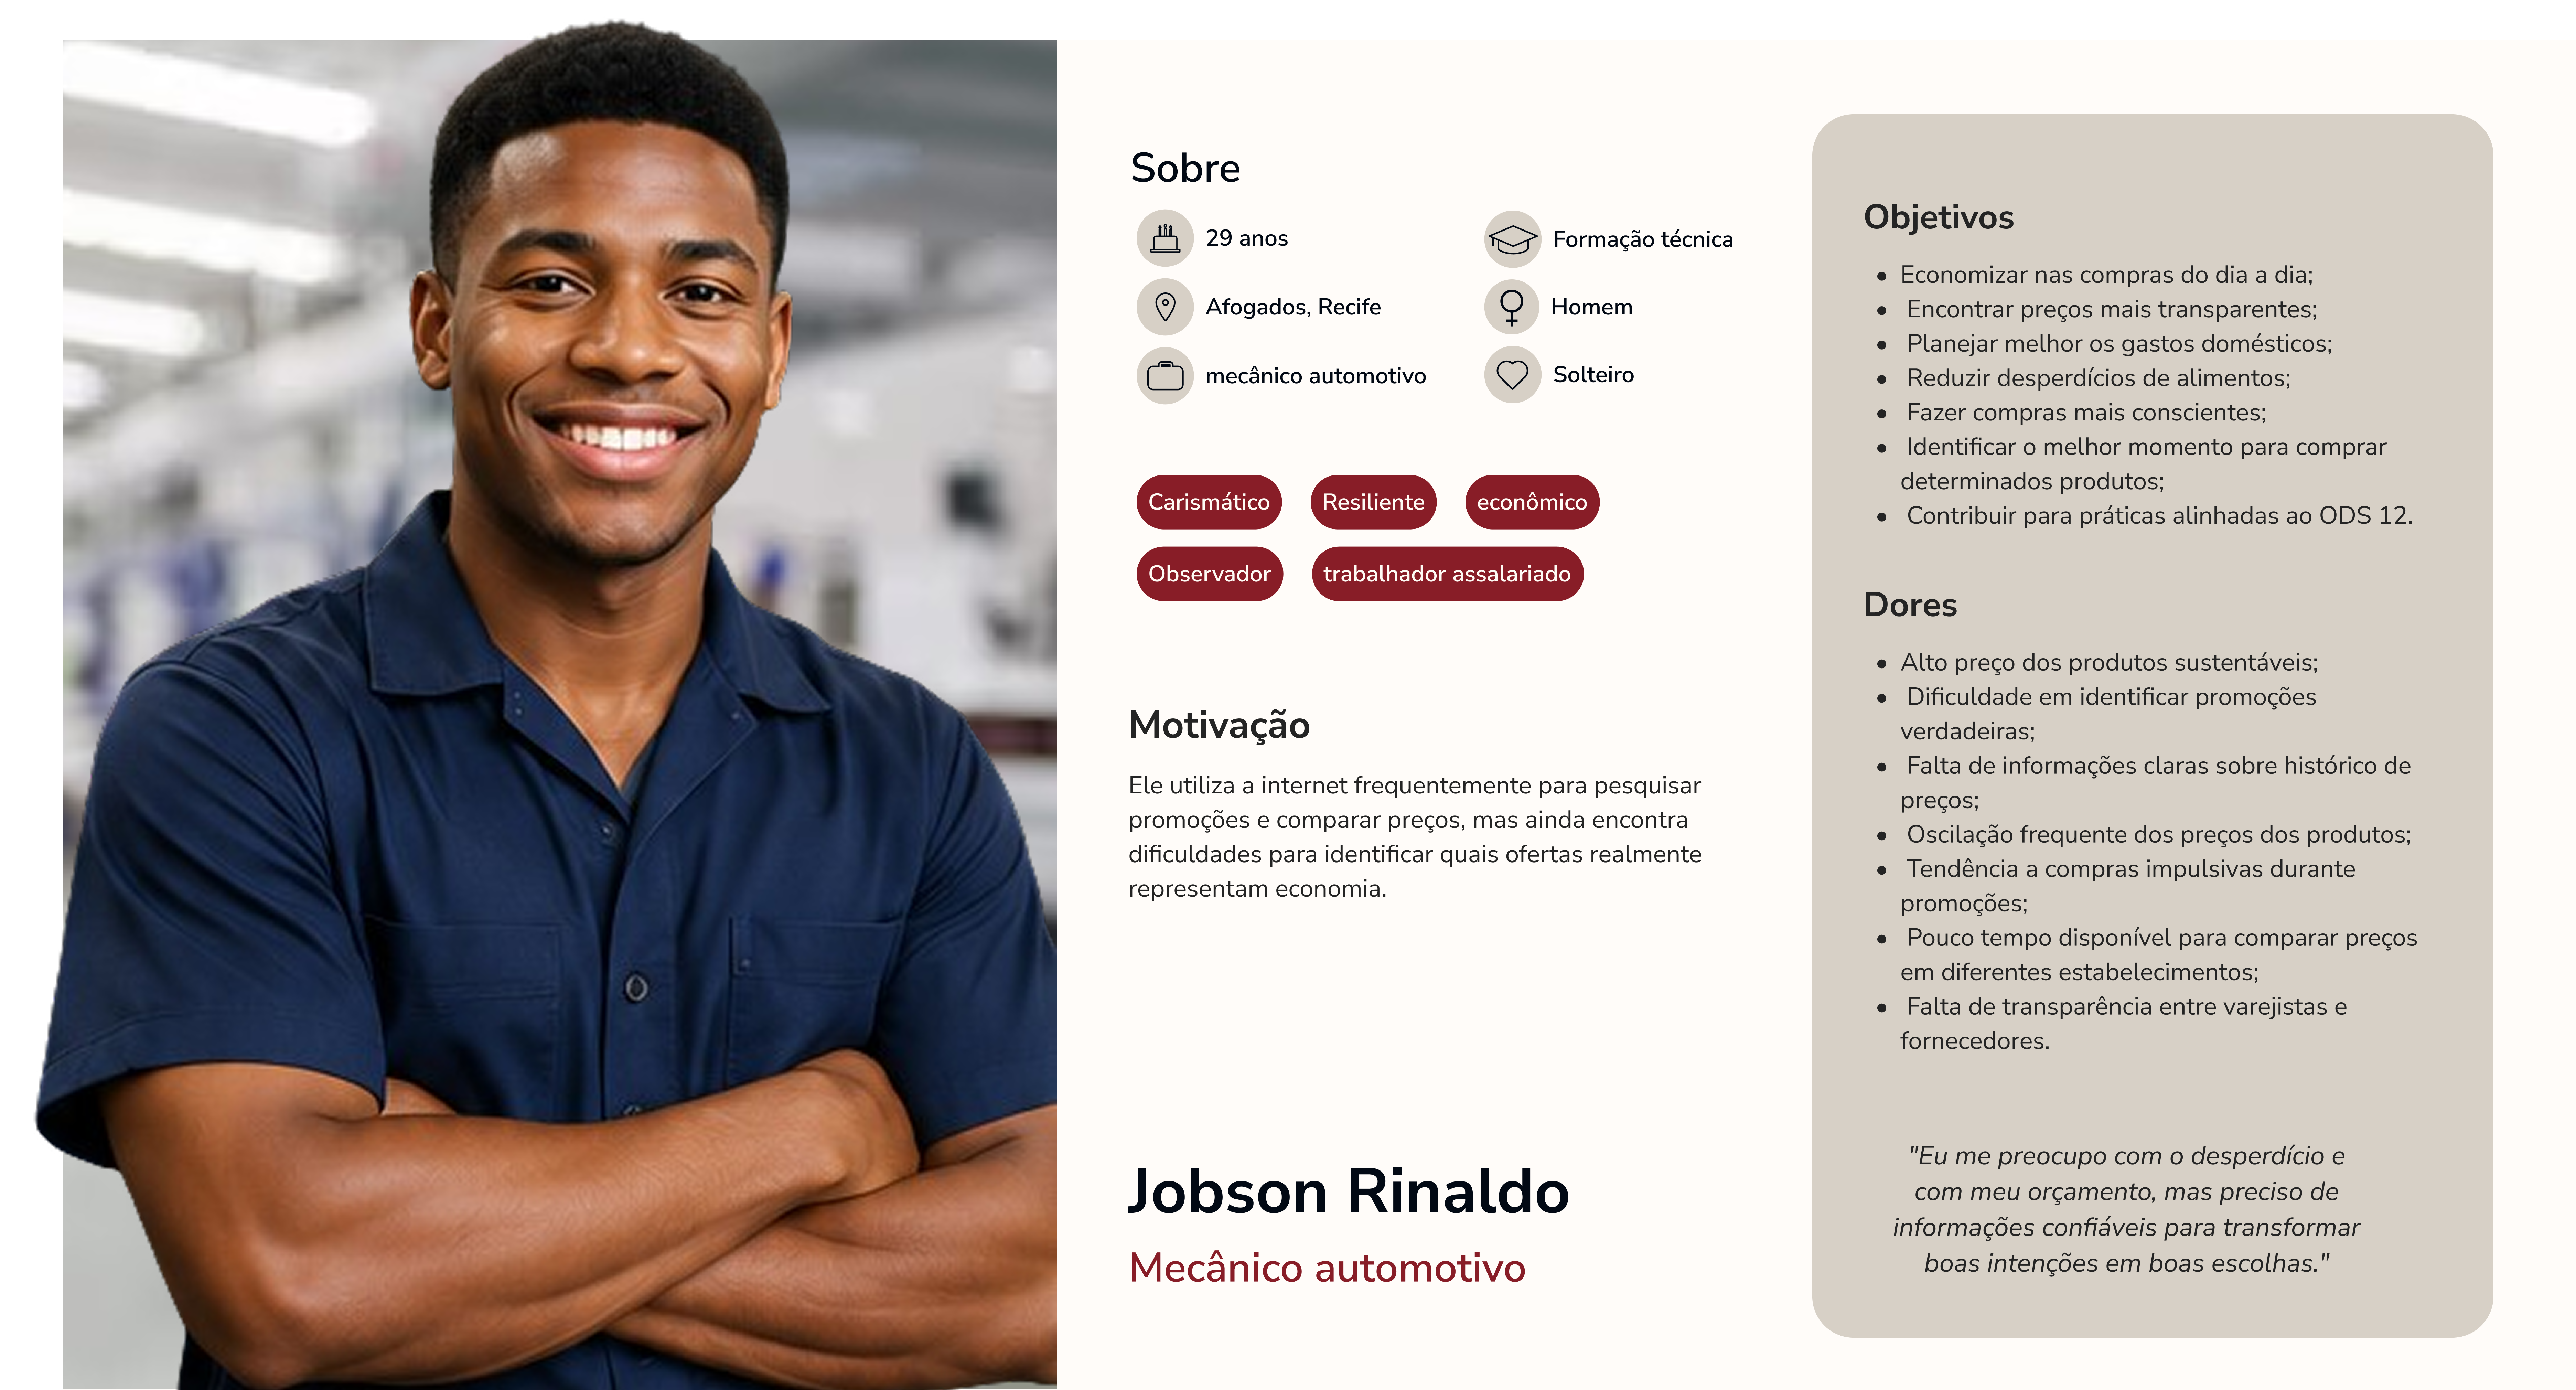
\includegraphics[width=\textwidth]{imgs/persona-jobson.png}
  \caption{Persona \textemdash{} Jobson Rinaldo, Mecânico Automotivo}
  \label{fig:persona-jobson}
\end{figure}

\begin{figure}[H]
  \centering
  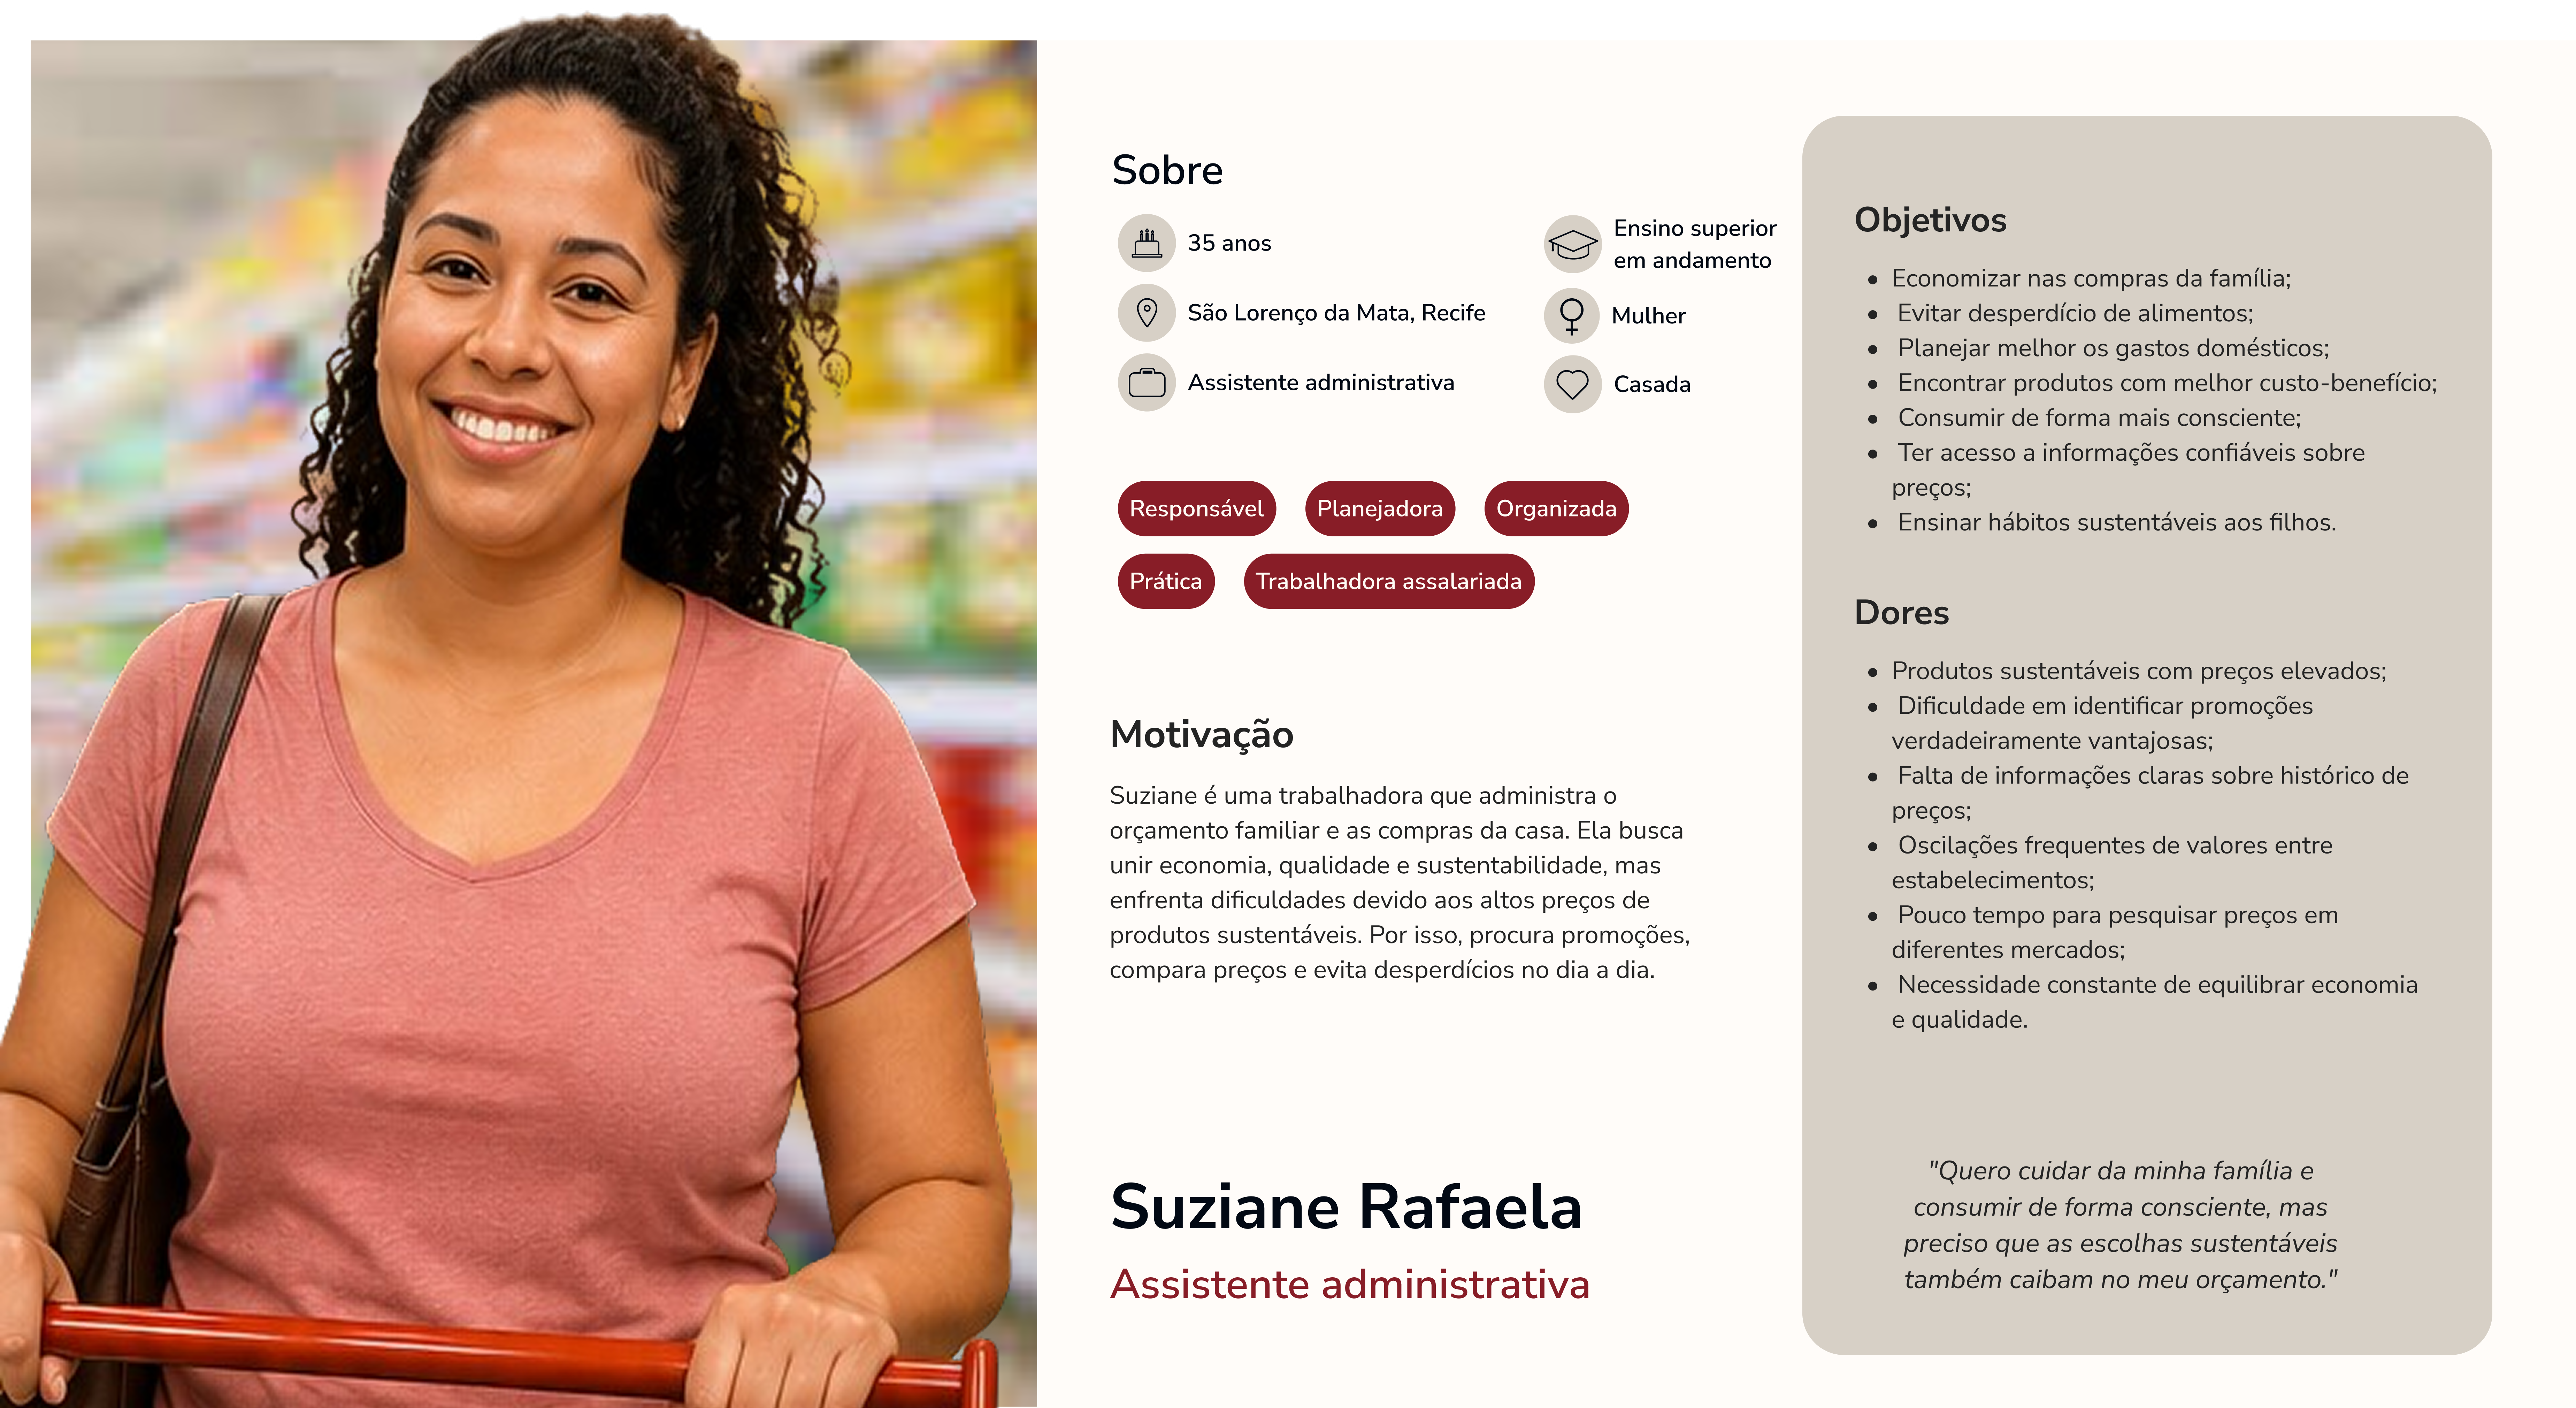
\includegraphics[width=\textwidth]{imgs/persona-suziane.png}
  \caption{Persona \textemdash{} Suziane Rafaela, Assistente Administrativa}
  \label{fig:persona-suziane}
\end{figure}

\subsection{Mapa de Empatia}

Os Mapas de Empatia foram construídos como ferramentas de síntese qualitativa, permitindo aprofundar a compreensão das experiências dos usuários para além dos dados numéricos obtidos na pesquisa.

\begin{figure}[H]
  \centering
  \includegraphics[width=\textwidth]{imgs/mapa-empatia-jobson.png}
  \caption{Mapa de Empatia \textemdash{} Jobson Rinaldo}
  \label{fig:empatia-jobson}
\end{figure}

\begin{figure}[H]
  \centering
  \includegraphics[width=\textwidth]{imgs/mapa-empatia-suziane.png}
  \caption{Mapa de Empatia \textemdash{} Suziane Rafaela}
  \label{fig:empatia-suziane}
\end{figure}

\subsection{Jornada do Usuário}

A Jornada do Usuário foi construída para representar a experiência atual dos consumidores \textbf{antes} da implementação da solução proposta, identificando os pontos de atrito e oportunidades de melhoria em cada fase do processo de compra.

\begin{itemize}[leftmargin=1.4em, itemsep=10pt]
  \item[\textcolor{wine}{\textbf{Antes}}] Os usuários pesquisam promoções, consultam encartes e planejam gastos, mas enfrentam dificuldades para avaliar se as ofertas encontradas realmente representam economia. \textit{Estado emocional: expectativa, cautela e incerteza.}

  \item[\textcolor{wine}{\textbf{Durante}}] Os consumidores comparam preços e tomam decisões com base nas informações disponíveis no momento. A ausência de histórico de preços gera insegurança e favorece compras impulsivas. \textit{Estado emocional: dúvida e indecisão.}

  \item[\textcolor{wine}{\textbf{Após}}] Os usuários avaliam os produtos adquiridos e refletem sobre suas escolhas. Muitas vezes encontram preços menores posteriormente ou percebem que poderiam ter planejado melhor. \textit{Estado emocional: alívio, reflexão e eventual frustração.}
\end{itemize}

% ============================================================================
%  6. CONSIDERAÇÕES FINAIS
% ============================================================================
\novaSecao{Considerações Finais}

A etapa de Imersão permitiu à Equipe ÉPSILON compreender de forma aprofundada a relação entre consumidores, informações de mercado e práticas de consumo consciente, alinhando a investigação aos princípios da ODS 12.

A combinação entre Pesquisa Desk, Questionário Online e Entrevistas Semiestruturadas possibilitou a obtenção de dados complementares, contribuindo para uma visão mais ampla do problema investigado. Os resultados evidenciaram que, embora exista interesse por práticas sustentáveis, fatores como a falta de informação, a dificuldade de acompanhar preços e os custos elevados ainda representam obstáculos significativos.

As personas, mapas de empatia e jornadas do usuário desenvolvidos ao longo desta etapa transformaram dados em conhecimento sobre os usuários, fortalecendo a compreensão de suas necessidades, comportamentos, dores e expectativas. Essas ferramentas serão fundamentais para orientar as próximas fases do projeto, garantindo que as soluções propostas estejam centradas nas necessidades reais do público-alvo.

\noindent{\sffamily\bfseries\color{wineDeep} Destaques da Imersão}
\vspace{4pt}

\begin{itemize}[leftmargin=1.2em, itemsep=4pt, label=\textcolor{wineSoft}{\textbf{\textbullet}}]
  \item \textbf{Preço como principal barreira:} os participantes apontaram o alto custo dos produtos sustentáveis como uma das maiores dificuldades para a adoção de práticas de consumo consciente.
  \item \textbf{Importância da informação:} a falta de transparência e de acompanhamento histórico dos preços foi identificada como fator que dificulta decisões de compra mais seguras.
  \item \textbf{Potencial para consumo consciente:} a maioria dos participantes já adota práticas de redução de desperdício e reutilização de recursos, demonstrando predisposição para comportamentos alinhados à ODS 12.
\end{itemize}

% ============================================================================
%  7. REFERÊNCIAS
% ============================================================================
\novaSecao{Referências}

\setlength{\parskip}{10pt}

\newcommand{\refnum}[1]{\textcolor{wineDeep}{\sffamily\bfseries[#1]}\ }

\refnum{1} MERCADO AMBIENTAL. \textbf{ODS 12: Consumo e Produção Responsáveis}. [S.l.], [s.d.]. Disponível em: \url{https://www.mercadoambiental.com.br/ods-12-consumo-e-producao-responsaveis}. Acesso em: 1 jun. 2026.

\refnum{2} UNIVERSIDADE FEDERAL DA FRONTEIRA SUL (UFFS). \textbf{Rotulagem de produtos e sua contribuição para o consumo consciente}. Chapecó, [s.d.]. Disponível em: \url{https://portaleventos.uffs.edu.br/index.php/SEPE-UFFS/article/view/24513}. Acesso em: 1 jun. 2026.

\refnum{3} ORGANIZAÇÃO DAS NAÇÕES UNIDAS (ONU). \textbf{Objetivos de Desenvolvimento Sustentável}. Nova Iorque, [s.d.]. Disponível em: \url{https://brasil.un.org/pt-br/sdgs}. Acesso em: 1 jun. 2026.

\refnum{4} IDEO U. \textbf{What is a Persona?} Cambridge, Massachusetts, [s.d.]. Disponível em: \url{https://www.ideou.com/blogs/inspiration/what-is-a-persona}. Acesso em: 7 jun. 2026.

\refnum{5} INTERACTION DESIGN FOUNDATION (IxDF). \textbf{Personas \textemdash{} A Simple Introduction}. Aarhus, Dinamarca, [s.d.]. Disponível em: \url{https://www.interaction-design.org/literature/topics/personas}. Acesso em: 7 jun. 2026.

\refnum{6} NIELSEN NORMAN GROUP. \textbf{Personas Make Users Memorable for Product Team Members}. Fremont, Califórnia, [s.d.]. Disponível em: \url{https://www.nngroup.com/articles/persona/}. Acesso em: 7 jun. 2026.

\refnum{7} INSTITUTO AKATU. \textbf{Consumo Consciente}. São Paulo, [s.d.]. Disponível em: \url{https://akatu.org.br}. Acesso em: 1 jun. 2026.

\refnum{8} INSTITUTO BRASILEIRO DE GEOGRAFIA E ESTATÍSTICA (IBGE). \textbf{Pesquisa de Orçamentos Familiares}. Rio de Janeiro, [s.d.]. Disponível em: \url{https://www.ibge.gov.br}. Acesso em: 1 jun. 2026.

\refnum{9} INSTITUTO DE PESQUISA ECONÔMICA APLICADA (IPEA). \textbf{Consumo Sustentável e Desenvolvimento Econômico}. Brasília, [s.d.]. Disponível em: \url{https://www.ipea.gov.br}. Acesso em: 1 jun. 2026.

\refnum{10} FUNDAÇÃO PROCON-SP. \textbf{Pesquisas de preços e orientação ao consumidor}. São Paulo, [s.d.]. Disponível em: \url{https://www.procon.sp.gov.br}. Acesso em: 1 jun. 2026.

\refnum{11} BRASIL. Ministério do Desenvolvimento e Assistência Social. \textbf{Agenda 2030 e os Objetivos de Desenvolvimento Sustentável}. Brasília, [s.d.]. Disponível em: \url{https://www.gov.br/mds}. Acesso em: 1 jun. 2026.

\refnum{12} UNIVERSIDADE FEDERAL DE SÃO CARLOS (UFSCar). \textbf{Hábitos de consumo e comportamento sustentável dos consumidores brasileiros}. São Carlos, 2023. Disponível em: \url{https://www.ufscar.br}. Acesso em: 1 jun. 2026.

\vspace{6pt}
\noindent{\sffamily\bfseries\color{wineDeep}\small Material autoral \textemdash{} entrega da Definição}
\vspace{2pt}

\refnum{13} GRUPO 13 (Curso Técnico em Desenvolvimento de Sistemas, ETE Cícero Dias). \textbf{ÉPSILON \textemdash{} Definição: consumo consciente e transparência de preços}: personas, mapas de empatia e jornada do usuário. Recife, 2026. Projeto de design elaborado no Figma.

\end{document}